Como se explicó en [ref a desarrollo o intro] debido a la aritmética finita de la computadora %TODO agregar ref
las operaciones pueden llegar a ser muy inestables \cite{arithmetic}.

Un pequeño ejemplo:

$$\begin{pmatrix}
    5 & -1 & -1 & -1 \\
    -1 & 4 & 0 & -1 \\
    -1 & 0 & 5 & -2 \\
    -1 & -1 & -2 & 6 \\
\end{pmatrix}$$

Luego de correr EG debería quedar:

$$\begin{pmatrix}
    5 & -1 & -1 & -1 \\
    0 & \frac{19}{5} & -\frac{1}{5} & -\frac{6}{5} \\
    0 & 0 & \frac{91}{19} & -\frac{43}{19} \\
    0 & 0 & 0 & \frac{396}{91} \\
\end{pmatrix}$$

Pero por culpa de la falta de precisión de los double queda:

$$\begin{pmatrix}
    5 & -1 & -1 & -1 \\
    0 & 3.8 & -0.2 & -1.2 \\
    0 & 0 & 4.78947 & -2.26316 \\
    0 & 0 & 0 & 4.35165 \\
\end{pmatrix}$$

Se puede ver que $\frac{396}{91} \cong 4.351648352$ teniendo una diferencia de $0.00000165$ con $4.35165$.
Difieren poco pero es un caso chico, este error se podría repetir y acarrear terminando en un valor en esa posición muy diferente al esperado, afectando así el ranking final.\\

Para experimentar sobre esto construimos una serie de partidos ficticios con el propósito de que la matriz quede con \textit{valores diferentes en su diagonal}, posiblemente este no sea el peor caso de error pero suponemos que es suficientemente malo. Para calcular el error absoluto, ya que no contamos con el valor esperado, utilizamos la factorización de Cholesky ya que es más estable. Cabe destacar que este método se puede aplicar ya que la matriz resulta simétrica y definida positiva\cite{CMMpaper}.\\
%The Cholesky method is available, because the matrices are not only (obviously) symmetric and real, but are also positive definite.

Yendo en detalle hicimos que cada equipo (1 a total-1) juegue $id$ cantidad de partidos, es decir, el equipo 1 juega un partido, el 2 dos, etc. Salvo el último equipo que va a jugar la cantidad que sea necesaria para cumplir con los partidos de los demás.

Como se puede observar en la figura \ref{fig:bienDiferenteEnDiagonal} aumenta el error a medida que aumenta la cantidad de equipos, lo cuál es esperable ya que se realizan más despejes y cuentas y se acarrea más el error.\\

\begin{figure}[H]
 \centering
 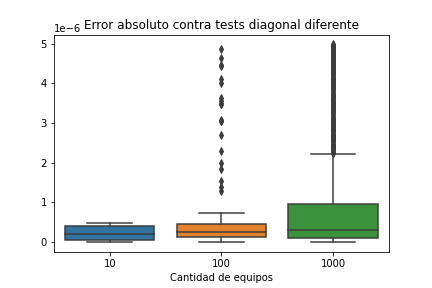
\includegraphics[scale=0.7]{imagenes/bienDiferenteEnDiagonal.png}
 \caption{Diferencia de error vs test diagonal diferente}
 \label{fig:bienDiferenteEnDiagonal}
\end{figure}

Luego, simplemente por probar otros casos decidimos utilizar el batch de tests generado por la cátedra. Al obtener los resultados notamos que los \textit{tests completos} generaban un error absoluto promedio mayor al que obtuvimos con nuestra \textit{diagonal diferente}, ver figura\ref{fig:testCatedra}.

Lo que suponíamos que podía estar pasando es que al haber muchos -1 al comienzo y no tantos 0s el error generado termina siendo mayor. Para probar esto hicimos nuestros propios tests de \textit{todos vs todos}, para diferentes cantidades de equipos. Pero al final, como se puede apreciar en la figura \ref{fig:todosVsTodos}, no pudimos llegar a un error tan grande como vs la cátedra. Suponemos que esto se debe a que nuestro oráculo no es tan estable como pensábamos y queda abierta la pregunta de cómo fueron calculados los resultados esperados para los casos de la cátedra.

\begin{figure}[H]
 \centering
 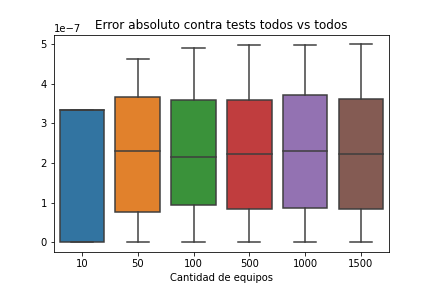
\includegraphics[scale=0.7]{imagenes/todosVsTodos.png}
 \caption{Diferencia de error vs test todos vs todos}
 \label{fig:todosVsTodos}
\end{figure}


\begin{figure}
\begin{subfigure}{.5\textwidth}
  \centering
  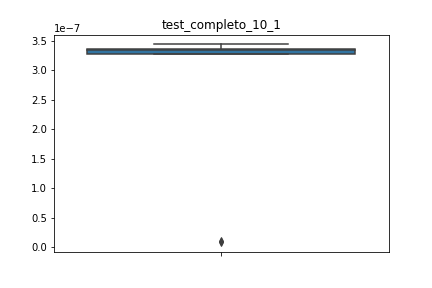
\includegraphics[width=\linewidth]{imagenes/test_completo_10_1.png}
\end{subfigure}%
\begin{subfigure}{.5\textwidth}
  \centering
  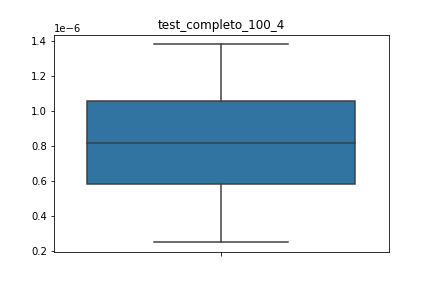
\includegraphics[width=\linewidth]{imagenes/test_completo_100_4.png}
\end{subfigure}
\begin{subfigure}{.5\textwidth}
  \centering
  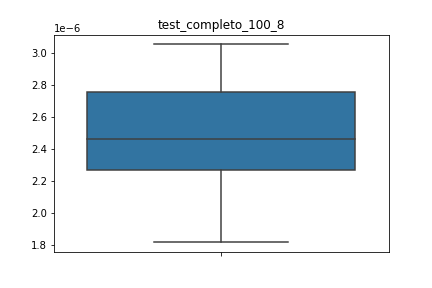
\includegraphics[width=\linewidth]{imagenes/test_completo_100_8.png}
\end{subfigure}%
\begin{subfigure}{.5\textwidth}
  \centering
  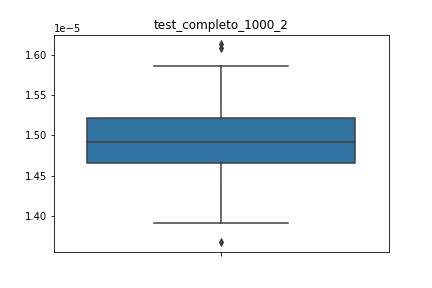
\includegraphics[width=\linewidth]{imagenes/test_completo_1000_2.png}
\end{subfigure}
\begin{subfigure}{.5\textwidth}
  \centering
  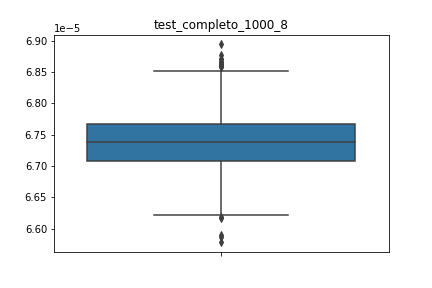
\includegraphics[width=\linewidth]{imagenes/test_completo_1000_8.png}
\end{subfigure}
\caption{Diferencia de error vs test completos de la catedra}
\label{fig:testCatedra}
\end{figure}

\FloatBarrier
